\documentclass[a4paper,11pt]{article}
\usepackage{multicol}
%\usepackage{multitoc}
%\usepackage{german}
%\usepackage{bibgerm}
\usepackage{amsmath}
\usepackage{amsfonts}
\usepackage{xspace}
\usepackage[body={148mm,240mm,nohead}]{geometry}
\usepackage[ansinew]{inputenc}
\usepackage{listings}
\usepackage{tikz}
\usepackage{hyperref}
\lstset{language=C++, basicstyle=\ttfamily,
  stringstyle=\ttfamily, commentstyle=\it, extendedchars=true}

\usepgflibrary{arrows}

\newcommand{\dune}{\textsc{Dune}\xspace}
\newcommand{\modulename}[1]{\texttt{#1}\xspace}

\title{The dune-localfunctions module}

\author{The \dune Team}

\date{\today}

\begin{document}

\maketitle

\begin{abstract}
This document describes the \modulename{dune-localfunctions} module.
The module provides a C++ interface for shape functions needed in
finite element methods.  A growing list of implementations of this
interface is included. \modulename{dune-localfunctions}
is part of the Distributed and Unified Numerics Environment (\dune) which is
available from the site \url{http://www.dune-project.org/}.
\end{abstract}

\begin{multicols}{2}
{\small\tableofcontents}
\end{multicols}

\section{Introduction}

A feature common to all implementations of finite element methods are the
shape functions.  In the easier cases, these are polynomial functions
defined on a reference element and associated to some face of the reference
element.  The more complicated non-affine finite elements generalize this
by defining the shape functions directly on an element in the grid.

Implementations of shape functions are contained in all finite element codes,
but in most cases their implementation is so intertwined with the rest of
the code as to make their reuse in other situations impossible.
For the easier shape functions this may not matter much, as they are
fairly easy to implement.  Still, errors can occur and bugs in shape function
implementations can be difficult to detect and track down.
More exotic shape function implementations can get fairly involved
and require meticulous care to be done right.  For these reasons it is
very desirable to provide shape functions in a separate, reusable library.
This is what the \modulename{dune-localfunctions} module tries to do.


Following the UNIX philosophy of having each program doing only one thing,
but doing that thing well, the \modulename{dune-localfunctions} module
provides only local and global finite elements.  There are two sides to this.
\begin{enumerate}
 \item \modulename{dune-localfunction} prescribes an {\em interface} to shape functions.
  This interface
  should be general enough to encompass the needs of virtually all implementors
  of finite element codes.
 \item The module contains {\em implementations} of this interface.  The set
  of implementations contains common elements like the Lagrange elements and
  exotic ones as well.  We aim to collect contributions from outside sources
  and, in time, to be able to provide a shape function library that is virtually
  complete.
\end{enumerate}

\subsection{Static vs.\ Dynamic Interfaces}

From a textbook C++ perspective, an interface to finite element shape functions
can be described naturally using dynamical polymorphism.  An abstract base
class would describe all methods expected from a shape function implementation,
and actual implementations would derive from the base class.  Users of shape functions,
such as finite element assemblers, would receive shape function implementations
through pointers to the abstract base class.

However, the run-time overhead of virtual function calls is considered prohibitive
by some users.  We measured a slowdown of around 7\% when assembling a Laplace
stiffness matrix on a two-dimensional structured grid.  This can be relevant,
for example, in an explicit time-stepping method where a large percentage of
the overall time is spent assembling matrices.

We have therefore opted for a different way.  In \modulename{dune-localfunctions},
the implementation classes are {\em not} organized in a hierarchy.  Adherence
to a certain interface is enforced only implicitly, by a test suite.  Finite
element assemblers have to have the C++ type of the shape function implementation
as a template parameter, and can then call the object's methods directly.
The static interface is described in Section~\ref{sec:static_interface}.

Of course such a scheme makes it impossible to select shape function sets at run-time.
For example, $p$-adaptive methods, and methods on grids with more than a single
element type are precluded.  Therefore, \modulename{dune-localfunctions} offers
a second way to access its shape functions.  There is a set of {\em wrapper classes},
which are organized in a hierarchy using dynamical polymorphism.  These
wrapper classes are statically parametrized with a static implementation class
and forward the function calls to this implementation.  Details of this
{\em dynamic interface} are given in Section~\ref{sec:dynamic_interface}.

\subsection{Dependencies on other Modules}

When designing the \modulename{dune-localfunctions} module we have deliberately
tried to keep dependencies on other \dune modules to a minimum.  Ideally,
people should be able to use the shape functions from \dune without having
to use anything else from \dune.  The only exception here is \modulename{dune-common},
which all \dune modules depend on.

In addition to \modulename{dune-common}, \modulename{dune-localfunctions} currently
depends only on \modulename{dune-grid}.  This dependence is somewhat unfortunate,
and it has been hotly debated.  We would like users to be able to use \dune grids
without shapefunctions from \modulename{dune-localfunctions} and the shapefunctions
from \modulename{dune-localfunctions} without the grids from \modulename{dune-grid}.
While the former is easy, \modulename{dune-localfunctions} currently needs a few
features from \modulename{dune-grid} to work.  These are in particular a few
quadrature rules and some of the infrastructure for constructing reference elements.
More seriously, \modulename{dune-localfunctions} provides some {\em global} finite
elements (also known as {\em non-affine families} of finite elements).  These
have to have some information about the geometry of the grid.

In the future the necessary things from \modulename{dune-grid} may be split off
into a separate module \modulename{dune-geometry} (or similar).  The dependence of
\modulename{dune-localfunctions} on \modulename{dune-grid} can then be replaced
by the weaker dependency on the new module.


\section{The LocalFiniteElement Interface}
\label{sec:static_interface}

\subsection{The LocalBasis Classes}

\subsection{The LocalCoefficients Classes}

\subsection{The LocalInterpolation Classes}


\section{The Dynamic Interface}
\label{sec:dynamic_interface}

\section{Global Finite Elements}

So far this document has talked about finite elements on reference elements.
However, the finite element is usually needed on an element of a grid.  To
evaluate a function represented by a finite element basis on a particular grid
element $T$ with geometry $\mu$ we can use the following formula:
\begin{equation}
  u(x)=\sum_{i=0}^{N_T-1}c_iP_{T,i}\varphi_i(\mu^{-1}(x)) \qquad\forall x\in T
\end{equation}
The basis function $\varphi$ on the reference element is provided by the local
basis which was described previously.  The global basis takes this local basis
and applies an operator $P_{T,i}$ to the values it returns.  This operator is
dependent on the grid element $T$ and the number of the basis function $i$.
The global basis thus provides values of the global basis functions
\begin{equation}
  \Phi_i(\hat x)=P_{T,i}\varphi_i(\hat x)
\end{equation}

For the transformation $P$ the following information about grid element is
important:
\begin{enumerate}
\item The {\em geometry} $\mu$ of a grid element, which handles the
  transformation of coordinates from the reference element to the grid
  element.  But {\em values} of the base functions and in particular their
  derivatives need to be transformed as well in general -- the correct
  transformation depends on the family of the finite element, the coordinate
  transformation $\mu$ and the number of the base function $i$.
\item The {\em topology} $\tau$ of a grid element, which says how the grid
  elements vertices a globally numbered in comparison to the numbering in the
  reference element.  This is needed for vector valued finite elements such as
  Raviar-Thomas and edge-elements.  Here the dofs often have an orientation
  which can be chosen arbitrary but must match for all shape function of the
  same dof (but from different grid elements).
\end{enumerate}

This section explicitly does not deal with the following issues:
\begin{itemize}
\item Different geometry types for different grid elements.  This will lead to
  different number of basis functions and must already be dealt with in the
  local finite element.
\item $p$-adaptiviy.  Again, this will lead to different number of basis
  functions and must already be dealt with in the local finite element.
\item Renumbering of base functions.  This may be required for things like Q3
  which have multiple dofs on a given face and assign specific positions
  inside the face to those dofs.
\end{itemize}

\subsection{Geometry}

The geometry information must be provided by a class basically modelling the
interface of {\tt GenericGeometry::BasicGeometry} -- that includes
implementations of {\tt Geometry}.  The precise requirements are as follows:
\begin{lstlisting}[escapechar=\$]
struct Geometry
{
  // type information
  typedef $\em implementation-defined$ ctype;
  // local dimension
  static const std::size_t mydimension = $\em implementation-defined$;
  // global dimension
  static const std::size_t coorddimension = $\em implementation-defined$;
  // some vector type with mydimension components of type ctype
  typedef $\em implementation-defined$ LocalCoordinate;
  // some vector type with coorddimension components of type ctype
  typedef $\em implementation-defined$ GlobalCoordinate;
  // some matrix type with coorddimension x mydimension
  // components of type ctype
  typedef $\em implementation-defined$ JacobianInverseTransposed;
  // some matrix type with mydimension x coorddimension
  // components of type ctype
  typedef $\em implementation-defined$ JacobianTransposed;

  // general properties of the geometry
  GeometryType type() const;
  bool affine() const;

  // access to the coordinates of the corners
  std::size_t corners() const;
  GlobalCoordinate corner(std::size_t) const;

  // local to global and inverse mapping
  GlobalCoordinate global(const LocalCoordinate&) const;
  LocalCoordinate local(const GlobalCoordinate&) const;

  // access to Jacobian of the mapping
  const JacobianTransposed&
    jacobianTransposed(const LocalCoordinate&) const;
  const JacobianInverseTransposed&
    jacobianInverseTransposed(const LocalCoordinate&) const;

  // other information
  GlobalCoordinate center() const;
  ctype integrationElement(const LocalCoordinate&) const;
  ctype volume() const;
  GlobalCoordinate normal(std::size_t face,
                          const LocalCoordinate&) const;
};
\end{lstlisting}
For the exact meaning of these members look in the doxygen documentation for
{\tt Geometry} or {\tt GenericGeometry::BasicGeometry}.

The coordinate types ({\tt ctype}, {\tt mydimension}, {\tt coorddimension},
{\tt LocalCoordinate}, and {\tt GlobalCoordinate}) of a {\tt Geometry} object
provided when creating an instance of a finite element should coincide with
the coordinate types of that finite element's basis class.

\subsubsection{Gradient Transformation}

The transformation of a scalar function from the reference element to a grid
element using the geometry $\mu$ is trivial:
\begin{equation}
  \hat f(\hat x) = f(\mu(\hat x))
\end{equation}
The transformation of the gradient of such a function is a little bit more
complicated.  First we will need to employ the Jacobian, which we define for a
function $u$ as:
\begin{equation}
  J_u(x)=\begin{pmatrix}
    \partial_0u_0|_x     & \ldots & \partial_{n-1}u_0|_x \\
    \vdots               & \ddots & \vdots \\
    \partial_0u_{m-1}|_x & \ldots & \partial_{n-1}u_{m-1}|_x
  \end{pmatrix}
\end{equation}
This definition of the Jacobian lets us write a linear vector-valued function
$u$ in terms of its Jacobian $J_u$ as $u(x) = J_u \cdot x$.  For a scalar
valued function $f$ the gradient is the transpose of the Jacobian:
\begin{equation}
  \nabla f|_x = \begin{pmatrix}
    \partial_0f|_x \\ \vdots \\ \partial_{n-1}f|_x
  \end{pmatrix} = J_f^T(x)
\end{equation}
To do the actual transformation we employ the chain rule
\begin{equation}
  \hat J_{\hat f}({\hat x}) = J_f(\mu(\hat x))\cdot \hat J_\mu(\hat x)
\end{equation}
After transposing, left-multiplying by $\hat J_\mu^{-T}(\hat x)$ and replacing
the transposed Jacobians by gradient where applicable, we obtain
\begin{equation}
  \nabla f|_{\mu(\hat x)}
    = \hat J_\mu^{-T}(\hat x) \cdot \hat\nabla\hat f|_{\hat x}
\end{equation}

\subsubsection{Raviart-Thomas Elements -- Piola Transformation}

Raviart-Thomas elements are finite elements that ensure continuity of the
normal component across grid elements.  They do allow for jumps in the
tangential components, however.  For these elements, the degrees-of-freedom
(dofs) are usually associated with the face (sub-entity of codimension 1) on
which the normal component is non-zero.

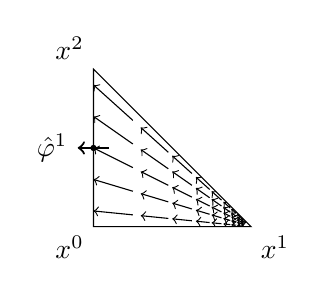
\begin{tikzpicture}[scale=2]
  \begin{scope}
    \draw[clip] (0,0) -- (1,0) -- (0,1) --cycle;
    \foreach \y in {.1,.3,...,.9}
      \foreach \x in {1,.7,.5,.35,.25,.175,.125,.0875,.0625}
        \draw[<-] (1-\x,\y*\x) -- +(\x/4,-\y*\x/4);
  \end{scope}
  \path (0,0) node[below left] {$x^0$}
        (1,0) node[below right] {$x^1$}
        (0,1) node[above left] {$x^2$};
  \draw[->,thick] (.1,.5) -- (-.1,.5) node[left] {$\hat\varphi^1$};
  \fill (0,.5) circle (.02);
\end{tikzpicture}

These elements have the following property:
\begin{equation}
  \varphi^i(x)\cdot n^j=\delta_{ij}\quad\forall x\in\text{face $j$}
\end{equation}
Here $n^j$ is the outer normal unit vector to face $j$ and $\delta_{ij}$ is
the Kronecker delta.  Naturally, transforming the basis should preserve that
property.  This is achieved by the Piola-transformation:
\begin{equation}
  \varphi^i(\mu(\hat x)) = \frac{\hat J_\mu(\hat x)}{|\hat J_\mu(\hat x)|}
    \hat\varphi^i(\hat x)
\end{equation}

\subsubsection{Edge Elements}

Edge elements are used in finite element electro-magnetics.  In the lowest
order, their dofs are associated with edges, i.e.\ sub-entities of dimension
1.  They can be expressed in terms of first order node-based Lagrange finite
elements $L^i$ as follows:
\begin{equation}
  N^i = \ell^i(L^{i_0} \nabla L^{i_1} - L^{i_1} \nabla L^{i_0})
\end{equation}
Here $i_0$ and $i_1$ are the indices of the nodes at the endpoints of edge $i$ and
$\ell^i$ is the length of edge $i$.

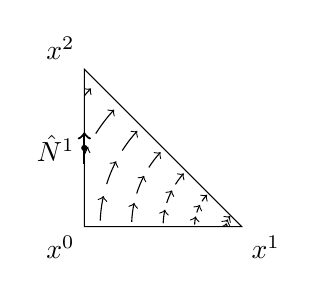
\begin{tikzpicture}[scale=2]
  \begin{scope}
    \draw[clip] (0,0) -- (1,0) -- (0,1) --cycle;
    \foreach \x in {.1,.3,...,1.5}
      \foreach \a in {2.5,17.5,32.5}
        \draw[->] (1,0) +(180-\a:\x) arc(180-\a:170-\a:\x);
  \end{scope}
  \path (0,0) node[below left] {$x^0$}
        (1,0) node[below right] {$x^1$}
        (0,1) node[above left] {$x^2$};
  \draw[->,thick] (0,.4) -- (0,.6);
  \fill (0,.5) circle (.02) node[left] {$\hat N^1$};
\end{tikzpicture}

Edge elements have a similar property as Raviart-Thomas elements: the
tangential component is 1 on the associated edge and 0 on all other edges:
\begin{equation}
  N^i(x)\cdot t^j=\delta_{ij}\quad\forall x\in\text{edge $j$}
\end{equation}

For the transformation we make the ansatz
\begin{equation}
  N^i(\mu(\hat x)) = \alpha^iA\hat N^i(\hat x)
\end{equation}
with the scalars $\alpha^i$ and a matrix $A$.  We express $N^i$ and $\hat N^i$
in terms of the corresponding P1 bases
\begin{equation}
  \ell^i\{L^{i_0}(\mu(\hat x)) \cdot \nabla L^{i_1}|_{\mu(\hat x)}
          - L^{i_1}(\mu(\hat x)) \cdot \nabla L^{i_0}|_{\mu(\hat x)}\}
  = \alpha^iA\hat\ell^i\{
          \hat L^{i_0}(\hat x) \cdot \hat\nabla\hat L^{i_1}|_{\hat x}
        - \hat L^{i_1}(\hat x) \cdot \hat\nabla\hat L^{i_0}|_{\hat x}\}
\end{equation}
By replacing the global P1 bases by the their transformations
\begin{align}
  L^i(\mu(\hat x)) &= \hat L^i(\hat x) \\
  \nabla L^i|_{\mu(\hat x)} &= \hat J_\mu^{-T}(\hat x) \hat\nabla\hat L^i|_{\hat x}
\end{align}
we obtain
\begin{multline}
  \ell^i\hat J_\mu^{-T}(\hat x)\{
          \hat L^{i_0}(\hat x) \cdot \hat\nabla\hat L^{i_1}|_{\hat x}
        - \hat L^{i_1}(\hat x) \cdot \hat\nabla\hat L^{i_0}|_{\hat x}\} \\
  = \alpha^iA\hat\ell^i\{
          \hat L^{i_0}(\hat x) \cdot \hat\nabla\hat L^{i_1}|_{\hat x}
        - \hat L^{i_1}(\hat x) \cdot \hat\nabla\hat L^{i_0}|_{\hat x}\}
\end{multline}
The expression inside the curly braces on both sides is the same.  We identify
\begin{align}
  A &= \hat J_\mu^{-T}(\hat x) \\
  \alpha^i &= \ell^i/\hat\ell^i
\end{align}
The full transformation then looks like this:
\begin{equation}
  N^i(\mu(\hat x)) = \frac{\ell^i}{\hat\ell^i}
    \hat J_\mu^{-T}(\hat x) \cdot \hat N^i(\hat x)
\end{equation}
Note that this transformation only works for the base functions, not for
superpositions of them.  Each base function $N^i$ has a different
transformation because the base multiplier $\alpha^i$ depends on the number of
the base function.

\subsubsection{Conclusions}

From the examples above we can conclude that the following information is
needed from a {\tt Geometry} class.  It is quite possible that the list below
is incomplete since the examples above may have missed some piece of
information that may be needed in general.
\begin{itemize}
\item The inverse transposed of the Jacobian $\hat J_\mu^{-T}(\hat x)$.
\item The Jacobian itself $\hat J_\mu(\hat x)$.
\item The determinant of the Jacobian $|\hat J_\mu(\hat x)|$.
\item The lengths of the edges of the grid element $\ell^i$.
\item The lengths of the edges of the reference element $\hat\ell^i$.
\end{itemize}
When local coordinates $\hat x$ are provided the local-to-global map $\mu(\hat
x)$ and its inverse $\mu^{-1}(x)$ as well as the corner coordinates $x^i$
themselves are never needed.  This makes the required information independent
of a shift in the global coordinates and opens an optimisation possibility for
regular grids.

\subsection{Topology}

The topology information is based completely on the global numbering of the
vertices of a grid element.  To obtain it, we collect the global IDs of the
vertices in a vector indexed by the indices of the vertices within the
reference element:
\begin{lstlisting}
void collectVertexIds(const Element& e, const GlobalIdSet& idSet,
                      std::vector<GlobaIdSet::IdType>& ids) {
  ids.resize(e.geometry().corners());
  for(int i = 0; i < ids.size(); ++ids)
    ids[i] = idSet.subId(e, i, Element::dimension);
}
\end{lstlisting}
In the next step the {\em topological reduction} operation is applied: the
smallest id in the array is replaced by the number 0, the second-smallest is
replaced by the number 1 etc.
\begin{lstlisting}
template<class LessThanComparable>
void topologicalReduction(const std::vector<LessThanComparable>& ids,
                          std::vector<std::size_t>& reduced) {
  std::vector<std::pair<LessThanComparable,std::size_t> > list(ids.size());
  for(std::size_t i = 0; i < ids.size(); ++i)
    list[i] = std::make_pair(ids[i], i);
  std::cout << list << std::endl;
  std::sort(list.begin(), list.end());
  std::cout << list << std::endl;
  reduced.resize(list.size());
  for(std::size_t i = 0; i <= list.size(); ++i)
    reduced[list[i].second] = i;
}
\end{lstlisting}
As an example, lets assume we have a quadrilateral or a tetrahedron with the
global ids of the vertices being 14 for vertex 0, 27 for vertex 1, 3 for
vertex 2 and 800 for vertex 3.  After topological reduction the reduced vector
will contain 1, 2, 0 and 3 in that order.

To ensure continuity for vector finite elements, we need to assign an
orientation to sub-entities shared by neighbouring grid elements.  Ideally,
this will work even if both neighbouring grid elements are of different
geometry type.

There is a distinction between local and global orientation: the local
orientation is the orientation according to the indices of the sub-entity's
vertices in the reference element.  The global orientation is the orientation
according to the global ids of the sub-entity's vertices within the grid.  If
the two orientations differ for a given grid element, the basis functions for
dofs on that sub-entity must be multiplied by $-1$.

\subsubsection{Line Orientation in 2D}

In 2D, the interface between two neighbouring elements is always a line.  For
lines in 2D there are however two different meanings of the term orientation,
depending on the finite element family.  Edge elements orient their dof along
the line, while Raviar-Thomas elements orient their dof perpendicular to the
line.  These two meaning are however compatible: the perpendicular orientation
can be obtained by turning the parallel orientation by $\pi/2$.  The rotation
must be perpendicular to the 2D-plane and should not flip -- this can be
achieved even for 2D manifold in a 3D space, unless you use something like a
M�bius strip.

The orientation of lines in 2D is from the lower index/id to the higher
index/id.

\subsubsection{Line Orientation in 3D}

In 3D the double-meaning of orientation does not occur.  This is not out of
principle, but just because I can only come up one family of finite elements
requiring orientation: edge elements.  The orientation of lines in 3D is
determined in the same way as for 2D: it is from the lower index/id to the
higher index/id.

\subsubsection{Triangle Orientation in 3D}

For 2D-entities in a 3D space we choose a face normal vector as the meaning of
the orientation.  If you look at a triangle and the reduced indices/ids of the
vertices run clockwise, the orientation vector points away from you, otherwise
it points towards you:

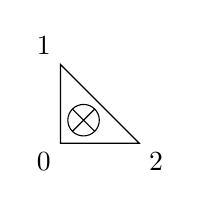
\begin{tikzpicture}
  \draw (0,0) node[below left] {0}
     -- (1,0) node[below right] {2}
     -- (0,1) node[above left] {1}
     --cycle;
  \coordinate (c) at (.29289,.29289);
  \draw (c) circle (.2);
  \draw (c) +(45:.2) -- +(45:-.2)
            +(-45:.2) -- +(-45:-.2);
\end{tikzpicture}
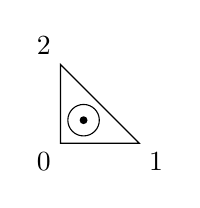
\begin{tikzpicture}
  \draw (0,0) node[below left] {0}
     -- (1,0) node[below right] {1}
     -- (0,1) node[above left] {2}
     --cycle;
  \coordinate (c) at (.29289,.29289);
  \draw (c) circle (.2);
  \fill (c) circle (.05);
\end{tikzpicture}

\subsubsection{Quadrilateral Orientation in 3D}

For quadrilaterals the numbering can be cyclic or acylic.  For the cyclic case
we choose the same rule as for the triangles: If you look at a triangle and
the reduced indices/ids of the vertices run clockwise, the orientation vector
points away from you, otherwise it points towards you.

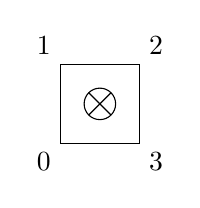
\begin{tikzpicture}
  \draw (0,0) node[below left] {0}
     -- (1,0) node[below right] {3}
     -- (1,1) node[above right] {2}
     -- (0,1) node[above left] {1}
     --cycle;
  \coordinate (c) at (.5,.5);
  \draw (c) circle (.2);
  \draw (c) +(45:.2) -- +(45:-.2)
            +(-45:.2) -- +(-45:-.2);
\end{tikzpicture}
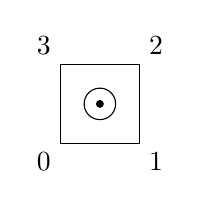
\begin{tikzpicture}
  \draw (0,0) node[below left] {0}
     -- (1,0) node[below right] {1}
     -- (1,1) node[above right] {2}
     -- (0,1) node[above left] {3}
     --cycle;
  \coordinate (c) at (.5,.5);
  \draw (c) circle (.2);
  \fill (c) circle (.05);
\end{tikzpicture}

The other possiblity is that the indices/ids run in the shape of the letter
``N'' or in the shape of its image mirrored at the diagonal
``\reflectbox{\rotatebox{90}{N}}''.  For the former case we choose orientation
away from the observer.  For the latter case we must then choose orientation
towards the observer.

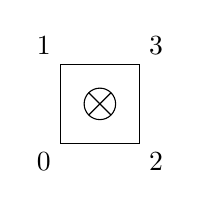
\begin{tikzpicture}
  \draw (0,0) node[below left] {0}
     -- (1,0) node[below right] {2}
     -- (1,1) node[above right] {3}
     -- (0,1) node[above left] {1}
     --cycle;
  \coordinate (c) at (.5,.5);
  \draw (c) circle (.2);
  \draw (c) +(45:.2) -- +(45:-.2)
            +(-45:.2) -- +(-45:-.2);
\end{tikzpicture}
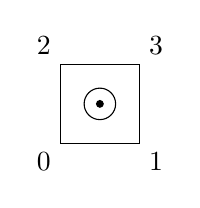
\begin{tikzpicture}
  \draw (0,0) node[below left] {0}
     -- (1,0) node[below right] {1}
     -- (1,1) node[above right] {3}
     -- (0,1) node[above left] {2}
     --cycle;
  \coordinate (c) at (.5,.5);
  \draw (c) circle (.2);
  \fill (c) circle (.05);
\end{tikzpicture}

Note that if you omit the index/id with the value 3 both the cyclic and the
acyclic case reduce to the triangle case.

\subsection{API}

The API for global-valued finite elements consists of five interface classes
({\tt Global\-Value\-Basis\-Interface}, {\tt
  GlobalValueInterpolationInterface}, {\tt
  Global\-Value\-Coefficients\-Interface}, {\tt
  GlobalValueFiniteElementInterface}, and {\tt
  Global\-Value\-Finite\-Element\-Factory\-Interface}) and two traits classes
({\tt GlobalValueBasisTraits} and {\tt
  Global\-Value\-Finite\-Element\-Traits}).  The name prefix ``{\tt
  GlobalValue}'' was chosen because these finite elements deal with global
base function values, but still take local coordinates on the reference
element.

\subsubsection{Finite Element Interface}

\begin{lstlisting}[escapechar=\$]
struct GlobalValueFiniteElementInterface
{
  // types of component objects
  struct Traits
  {
    typedef $\em implementation-defined$ Basis;
    typedef $\em implementation-defined$ Coefficients;
    typedef $\em implementation-defined$ Interpolation;
  };

  // construction
 private:
  // constructor *may* be private
  GlobalValueFiniteElementInterface(...);
 public:
  // ... except for the copy constructor
  GlobalValueFiniteElementInterface
    (const GlobalValueFiniteElementInterface&);

  // extract component objects
  const typename Traits::Basis& basis() const;
  const typename Traits::Coefficients& coefficients() const;
  const typename Traits::Interpolation& interpolation() const;
  GeometryType type() const;
};
\end{lstlisting}
The member class {\tt Traits} may be a member typedef instead.  Constructor
signatures and existence is implementation-defined, except for the copy
constructor, which must be present and publicly accessible.  Construction is
generally done by a factory class.  To keep copy-construction efficient it is
recommended that instanced of this class are light proxy objects.

The reason to mandate copy-construction is as follows: Up to now with local
finite elements \modulename{dune-pdelab} used the class {\tt FiniteElementMap}
as a kind of finite element factory.  If the finite element was required in
different variants for a given grid (i.e.\ because normal continuity was
required for Raviar-Thomas elements), the {\tt FiniteElementMap} would store
all the variants internally and return a reference to the correct variant upon
request.  Since global-valued finite elements depend on the geometry of the
grid element, this trick is no longer useful, especially if you plan to modify
the finite element object by ``binding'' it to the geometry.  The problem is
that more than one finite element for different grid elements may be required
at the same time (think iterating over the intersections).  If the {\tt
  FiniteElementMap} returns the same variant for both grid elements the user
code will first bind the finite element to the inside element and later to the
outside element, since both of his finite element references point to the same
object.  Thus when he tries to access the inside finite element, he will in
reality access the outside element.

\subsubsection{Finite Element Factory Interface}

\begin{lstlisting}[escapechar=\$]
enum Tristate { maybe = true+1 };
typedef std::vector<std::size_t> Topology;

template<class Geometry>
struct GlobalValueFiniteElementFactoryInterface
{
  // may also be an inline class
  typedef $\em implementation-defined$ FiniteElement;

  // construction is implementation-defined
  GlobalValueFiniteElementFactoryInterface(...);

  // finite element object creation
  const FiniteElement make();
  const FiniteElement make(const Topology&);
  const FiniteElement make(const Geometry&);
  const FiniteElement make(const Geometry&, const Topology&);

  // compile-time interface selection
  static const Tristate staticNeedGeometry = $\em implementation-defined$;
  static const Tristate staticNeedTopology = $\em implementation-defined$;

  // run-time interface selection
  bool needGeometry() const;
  bool needTopology() const;
};
\end{lstlisting}
The method to create a finite element object is {\tt make()}.  The created
object is returned by value ({\tt const FiniteElement}).  The factory
implementation may choose to return by reference instead ({\tt const
  FiniteElement\&}).  Because temporaries may be bound to const references in
C++, this way code using the factory can always bind the returned value to a
const reference and avoid copy construction if that is not necessary:
\begin{lstlisting}
const Factory::FiniteElement& fe = factory.make(geo, topo);
\end{lstlisting}
In any case, the returned value or reference must be valid for as long as the
factory object exists.

The different signatures for {\tt make()} exists for optimisation.  The
methods {\tt need\-Geometry()} and {\tt needTopology()} exists so code can
generically decide whether to do the possibly expensive computation geometry
and/or topology information.  Even if geometry or topology information is not
needed, it is always valid to provide it, in that case the arguments provided
to {\tt make()} is ignored.  If geometry or topology information has been
provided to the constructor of the factory and again to {\tt make()}, the
information provided to the constructor is used and consistency is not
checked.  If too little information is provided to make it should throw an
exception or an assertion.

In addition, some factories may know at compile time whether geometry or
topology information is needed or not.  They can export this knowledge via
{\tt staticNeedGeometry} and {\tt staticNeedTopology}.  If that knowledge is
not available at compile time, these constants must have the value {\tt
  maybe}.  Even if it can be determined at compile time that geometry and
topology information is needed, the signatures of {\tt make()} without those
arguments must still be present (and must throw an exception or assertion).

Implementations must document when geometry and topology information is
required.

The constructor signature is implementation-defined.

It is recommended that the factory caches as much information as possible.
For instance, for regular hypercube grids the Jacobian of the geometry does
not change and is the only thing needed to transform the derivatives.  For
this case the constructor should take a sample geometry and precompute the
transformation.  Whether the regular and the general case are distinguished by
different constructor arguments to the same factory class, or whether there is
one factory class for the regular and one for the general case is left to the
implementor of the factory.

\subsubsection{Basis Interface}
\begin{lstlisting}[escapechar=\$]
struct GlobalValueBasisInterface
{
  struct Traits
  {
    // domain properties (local and global)
    typedef $\em implementation-defined$ DomainField;
    static const std::size_t dimDomainLocal = $\em implementation-defined$;
    static const std::size_t dimDomainGlobal = $\em implementation-defined$;
    typedef $\em implementation-defined$ DomainLocal;
    typedef $\em implementation-defined$ DomainGlobal;

    // range properties (global range only)
    typedef $\em implementation-defined$ RangeField;
    static const std::size_t dimRange = $\em implementation-defined$;
    typedef $\em implementation-defined$ Range;

    // jacobian properties (dimRange x dimDomainGlobal Matrix with
    // components of type RangeField)
    typedef $\em implementation-defined$ Jacobian;

    // maximum number of partial derivatives supported
    static const std::size_t diffOrder = $\em implementation-defined$;
  };

  // Number of shape functions
  std::size_t size () const;
  // Polynomial order of the shape functions for quadrature
  std::size_t order () const;

  // Evaluate all shape functions at given position
  void evaluateFunction
  ( const typename Traits::LocalDomain& in,
    std::vector<typename Traits::Range>& out) const;

  // Evaluate jacobian of all shape functions at given position
  // required for Traits::diffOrder >= 1
  void evaluateJacobian
  ( const typename Traits::LocalDomain& in,
    std::vector<typename Traits::Jacobian>& out) const;

  // Evaluate derivatives of all shape functions at given position
  // required for Traits::diffOrder >= 2
  void evaluate
  ( const array<std::size_t,Traits::dimGlobalDomain>& directions,
    const typename Traits::LocalDomain& in,
    std::vector<typename Traits::Range>& out) const;
};
\end{lstlisting}
The basis interface closely follows the local basis interface with some
notable exceptions.

First the are the types in the traits class.  Since coordinates are sill given
in the reference elements coordinate system but derivatives are done with
respect to global coordinates, a distinction must be made between local and
global domain.  The other change is that the member types of the traits class
no longer have a suffix ``{\tt Type}'' since it is quite clear from the
camel-case naming convention that they are types.

Second the method for general derivatives {\tt evaluate()} is no longer a
template method and its argument {\tt directions} has different semantics.  In
the local basis interface, {\tt directions} was a list of directions in which
to take derivatives, i.e.\ {\tt directions=\{0, 1, 0, 2\}} for the derivative
$\partial_0\partial_1\partial_0\partial_2$.  This is inconvenient since it
requires {\tt directions} to be a list of variable length, making the length a
template parameter, and because the order implied in the above derivative does
not really exist, it can just as well be written as
$\partial_0^2\partial_1\partial_2$.  So in the global-value interface {\tt
  directions} lists the exponents in the last expression: {\tt direction=\{2,
  1, 1\}}.  This way the length of {\tt directions} will always be {\tt
  Traits::dimDomainGlobal} and {\tt evaluate()} no longer needs to be a
template.

\subsubsection{Interpolation Interface}

\begin{lstlisting}
struct GlobalValueInterpolationInterface
{
  // Export basis traits
  typedef GlobalValueBasisInterface::Traits Traits;

  // determine coefficients interpolating a given function
  template<typename F, typename C>
  void interpolate (const F& f, std::vector<C>& out) const;
};
\end{lstlisting}
The interface for global-value interpolation objects also has little
modifications compared to local interpolation objects.  Main addition is the
member type {\tt Traits} which is the same as in the corresponding basis
class.  This is to document the parameter types that {\tt interpolate()} will
use to evaluate the function {\tt f}.

For the member method {\tt evaluate()} the requirements for the function
object {\tt f} change slightly: it is still required to support the expression
{\tt f.evaluate(x, y)}, and {\tt x} in that expression is still a local
coordinate (though the type is named a little bit different: {\tt const
  Traits::DomainLocal\&}.  The difference is that the returned value {\tt y}
is now in global coordinates and of the type {\tt Traits::Range}.

\subsection{Coefficients Interface}

\begin{lstlisting}
struct GlobalValueCoefficientsInterface
{
  // number of coefficients
  std::size_t size() const;

  // get i'th index
  const LocalKey& localKey(std::size_t i) const;
};
\end{lstlisting}
The interface for the coefficients class is exactly the same as for the local
coefficients.  If the global-valued finite elements is implemented in term of
a local finite element it will often be possible to simply reuse the
coefficients class of the local finite element.

\section{Appendix: List of Available Elements}



% bibtex bibliography
%\bibliographystyle{plain}
%\bibliography{istl.bib}


\end{document}
